\section{第一次迭代开发成果展示}
\begin{frame}{用户注册新账号}
    \begin{itemize}
        \item 用户故事描述:作为一个新用户,我想要注册一个新账号,以便于使用网站的各种功能和服务。
        \item 接口责任人:李其桐
        \item 功能页面设计: //TODO
    \end{itemize}
\end{frame}

\begin{frame}{用户登录账号}
    \begin{itemize}
        \item 用户故事描述:作为一个已注册的用户,我想要登录我的账号,以便于使用网站的各种功能和服务。
        \item 接口责任人:李其桐
        \item 附加信息:如果用户已登录,并且没有进行登出操作,则关闭页面后再登录系统时应当能够自动验证会话并且跳转到主页。
        \item 功能页面设计: //TODO
    \end{itemize}
\end{frame}

\begin{frame}{用户查看自身上传的模型文件}
    \begin{itemize}
        \item 用户故事描述:作为一个AI绘画软件系统使用者,我想要查看我上传的模型文件,以便于管理我的作品和修改我的设计。
        \item 接口责任人:李其桐
        \item 功能页面设计: //TODO
    \end{itemize}
\end{frame}

\begin{frame}{用户删除自身上传的模型文件}
    \begin{itemize}
        \item 用户故事描述:作为一个AI绘画软件系统使用者,我想要删除我上传的模型文件,以便于清理我的空间、避免重复或错误的作品、或者更新迭代我的模型文件版本。
        \item 接口责任人:吴达鹏
        \item 功能页面设计: //TODO
    \end{itemize}
\end{frame}

\begin{frame}{根据模型名字搜索模型}
    \begin{itemize}
        \item 用户故事描述:作为一个模型使用者,我想要根据模型名字搜索模型,以便于快速找到我需要的绘图模型和相关信息。
        \item 接口责任人:李其桐
        \item 功能页面设计: //TODO
    \end{itemize}
\end{frame}

\begin{frame}{根据用户名搜索用户}
    \begin{itemize}
        \item 用户故事描述:作为一个模型使用者,我想要根据用户名搜索用户,以便于关注我喜欢的模型训练师和随时查看他们的作品并且获取他们的动态。
        \item 接口责任人:陈骁
        \item 功能页面设计: //TODO
    \end{itemize}
\end{frame}

\begin{frame}{用户查看一个模型的所有评论}
    \begin{itemize}
        \item 用户故事描述:作为一个模型使用者,我想要查看一个模型的所有评论,以便于了解其他用户的反馈和建议。
        \item 接口责任人:刘昱彤
        \item 功能页面设计: //TODO
    \end{itemize}
\end{frame}

\begin{frame}{用户对于模型发表评论}
    \begin{itemize}
        \item 用户故事描述:作为一个模型使用者,我想要对一个模型发表评论,以便于表达我的意见和感受,以及和其他用户交流。
        \item 接口责任人:于采篱
        \item 功能页面设计: //TODO
    \end{itemize}
\end{frame}

\begin{frame}{用户删除已发表的评论}
    \begin{itemize}
        \item 用户故事描述:作为一个模型使用者,我想要删除我已发表的评论,以便于撤回我不想要的或错误的意见。
        \item 接口责任人:陈骁
        \item 功能页面设计: //TODO
    \end{itemize}
\end{frame}

\begin{frame}{用户点赞模型}
    \begin{itemize}
        \item 作为一个模型使用者,我想要点赞一个模型,以便于支持我喜欢的模型设计师和推荐优秀的模型给其他用户。
        \item 接口责任人:曾诗容
        \item 功能页面设计: %//TODO
        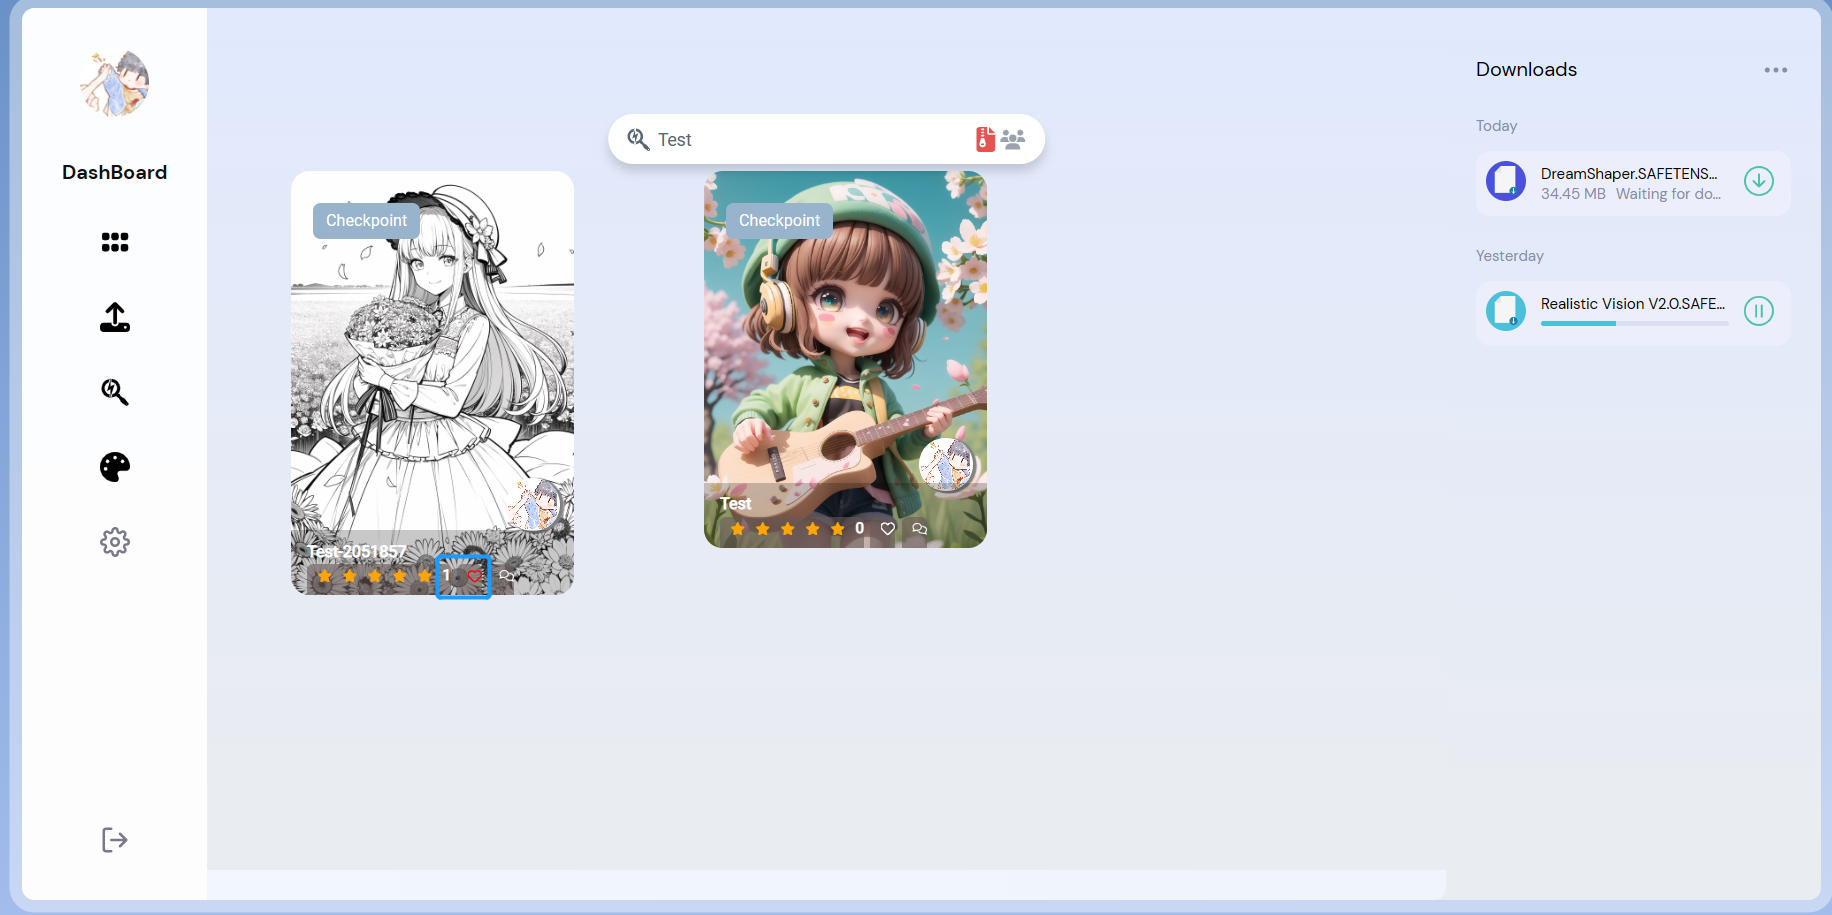
\includegraphics[width=3.8in]{contents/figure/like_model_demo.png}
    \end{itemize}
\end{frame}

\begin{frame}{用户取消对于一个模型的点赞}
    \begin{itemize}
        \item 用户故事描述:作为一个模型使用者,我想要取消对于一个模型的点赞,以便于更改我的喜好和评价。
        \item 接口责任人:林奕如
        \item 功能页面设计: //TODO
    \end{itemize}
\end{frame}

\begin{frame}{用户设置模型转换需求,如Prompt描述、图片尺寸、模型相关参数等等}
    \begin{itemize}
        \item 用户故事描述:作为一个模型使用者,我想要设置模型转换需求,如图片尺寸、模型相关参数等等,以便于根据我的具体需求和场景,定制化地使用模型。
        \item 接口责任人:陈骁
        \item 附加信息:转换需求设置应当能够加载网站中已有的模型文件,以便于用户能够快速地设置模型转换需求。
        \item 功能页面设计: //TODO
    \end{itemize}
\end{frame}

\begin{frame}{用户运行模型生成图片}
    \begin{itemize}
        \item 用户故事描述:作为一个模型使用者,我想要运行模型生成图片,以便于看到模型的效果和输出。
        \item 接口责任人:陈骁
        \item 功能页面设计: //TODO
    \end{itemize}
\end{frame}

\begin{frame}{用户登出}
    \begin{itemize}
        \item 用户故事描述:作为一个已登录的用户,我想要在我不需要使用软件系统的时候登出我的账号,以便于保护我的隐私和安全。
        \item 接口责任人:李其桐
        \item 功能页面设计: //TODO
    \end{itemize}
\end{frame}